\chapter{Clearing The Window}

In this chapter we see all the steps that are required to draw something
on our window.

First, during our application startup phase, we need to create some resources
required for rendering.
We create two semaphores to synchronize the execution of graphics and present
commands.
We create a command pool and allocate a command buffer from it.
Finally, we describe our rendering operations using a render pass.

Then, during our application main loop, we need to execute a set of steps
for our rendering and presenting to be correct.
We first acquire a swapchain image that will be used as our render target.
We wait for the previously submitted commands to finish their execution.
We bundle our swapchain image into a framebuffer, so that we can use it
during rendering.
At last we record graphics commands into our command buffer.
We submit the command buffer to our graphics queue.
Finally, we submit a present command to our present queue.

\section{Create Commands Synchronization Resources}

We have to manually synchronize the commands we use for rendering an image
and the commands we use for presenting said image to the window.
To do this we use two semaphores.
One semaphore will be signaled when a swapchain image is available to
be used as our render target.
Another semaphore will be signaled when we finish rendering our image.
Only after this semaphore has been signaled, we are allowed to present our
image to the window.

\begin{minipage}{\linewidth}{\noindent}
    \lstinputlisting[
        language=C++,
        caption={Create semaphores},
        label={lst::CreateSemaphores}
        ]{src/ChClearWindow/CreateSemaphores.cpp}
\end{minipage}

\subsection{Cleanup}

We destroy the previously allocated semaphores with vkDestroySemaphore.

\section{Create Graphics Command Pool}

Before submitting commands to a GPU queue, we need to create a command pool.
We will explicitly submit commands only to our graphics queue.
Hence, we create one graphics command pool.

\begin{minipage}{\linewidth}{\noindent}
    \lstinputlisting[
        language=C++,
        caption={Create graphics command pool},
        label={lst::CreateGraphicsCommandPool}
        ]{src/ChClearWindow/CreateGraphicsCommandPool.cpp}
\end{minipage}

\subsection{VkCommandPoolCreateInfo}

We use a VkCommandPoolCreateInfo struct to configure the command pool we are
about to create.
Here we use the reset command buffer flag because we want to be able to
write commands multiple times into the command buffers created from this pool.

\begin{minipage}{\linewidth}{\noindent}
    \lstinputlisting[
        language=C++,
        caption={Configure our graphics command pool},
        label={lst::VkCommandPoolCreateInfo}
        ]{src/ChClearWindow/VkCommandPoolCreateInfo.cpp}
\end{minipage}

\subsection{Cleanup}

When our application is shutting down we have to destroy all the previously created
command pools.
To do this we use vkDestroyCommandPool.

\section{Create Command Buffer}

We need a command buffer to submit commands to our GPU.
We allocate a command buffer from a command pool.

\begin{minipage}{\linewidth}{\noindent}
    \lstinputlisting[
        language=C++,
        caption={Allocate a command buffer from our graphics command pool},
        label={lst::AllocateCommandBuffer}
        ]{src/ChClearWindow/AllocateCommandBuffer.cpp}
\end{minipage}

\subsection{VkCommandBufferAllocateInfo}

We use a VkCommandBufferAllocateInfo struct to configure the command buffer we are
about to create.
In our case we allocate a primary command buffer.
Such buffers can be directly submitted to GPUs to be executed.

\begin{minipage}{\linewidth}{\noindent}
    \lstinputlisting[
        language=C++,
        caption={Configure command buffer creation},
        label={lst::VkCommandBufferAllocateInfo}
        ]{src/ChClearWindow/VkCommandBufferAllocateInfo.cpp}
\end{minipage}

\subsection{Command Buffer Fence}

Together with our command buffer, we also create a fence.
We can use a fence to wait for our command buffer execution to finish.
The fence that we create is already signaled from the start.
This is due to how we will use it later.

\begin{minipage}{\linewidth}{\noindent}
    \lstinputlisting[
        language=C++,
        caption={Create a fence for our command buffer},
        label={lst::CreateFence}
        ]{src/ChClearWindow/CreateFence.cpp}
\end{minipage}

\subsection{Cleanup}

We use vkFreeCommandBuffers to free the previously allocated command buffers.
We use vkDestroyFence to destroy our the previously created fences.

\section{Create Render Pass}

Before rendering, we need to describe what types of images will be used and the
order of our draw calls.
To do this we create a render pass.

\begin{minipage}{\linewidth}{\noindent}
    \lstinputlisting[
        language=C++,
        caption={Create a render pass},
        label={lst::CreateRenderPass}
        ]{src/ChClearWindow/CreateRenderPass.cpp}
\end{minipage}

\subsection{VkRenderPassCreateInfo}

We use a VkRenderPassCreateInfo struct to configure the render pass we
are about to create.

\begin{minipage}{\linewidth}{\noindent}
    \lstinputlisting[
        language=C++,
        caption={Configure our render pass},
        label={lst::VkRenderPassCreateInfo}
        ]{src/ChClearWindow/VkRenderPassCreateInfo.cpp}
\end{minipage}

\subsection{Render Pass Attachment Descriptions}

During render pass creation, we specify an array of attachment descriptions.
This array describes all the attachments that are going to be used by our
render pass.

In our case we have only one attachment.
This attachment will be one of the swapchain images.
Before using our attachment for the first time during our render pass, we clear it.
After using our attachment for the last time during our render pass, we preserve
its contents.
We don't care about the attachment's stencil components.
Before starting the render pass, we don't care about the attachment's image layout.
At the end of the render pass, we want to transition the attachment to a layout
compatible with image presentation.

\begin{minipage}{\linewidth}{\noindent}
    \lstinputlisting[
        language=C++,
        caption={Render pass attachment descriptions},
        label={lst::RenderPassAttachment}
        ]{src/ChClearWindow/RenderPassAttachments.cpp}
\end{minipage}

\subsection{Render Pass Subpasses}

During render pass creation, we specify an array of subpass descriptions.
This array describes the subpasses that define our render pass.

In our case we have only one subpass that uses our single attachment to write
color data into it.
In order to be able to write color data into our attachment we need it to have
a proper image layout.

\begin{minipage}{\linewidth}{\noindent}
    \lstinputlisting[
        language=C++,
        caption={Render pass subpass descriptions},
        label={lst::RenderPassSubpasses}
        ]{src/ChClearWindow/RenderPassSubpasses.cpp}
\end{minipage}

\subsection{Cleanup}

To destroy our render pass we use vkDestroyRenderPass.

\section{Clear The Window}

In our application, we render an image each iteration of our main loop.
In this case, we simply clear the window background with a flat color.

\begin{figure}[ht]
    \centering
    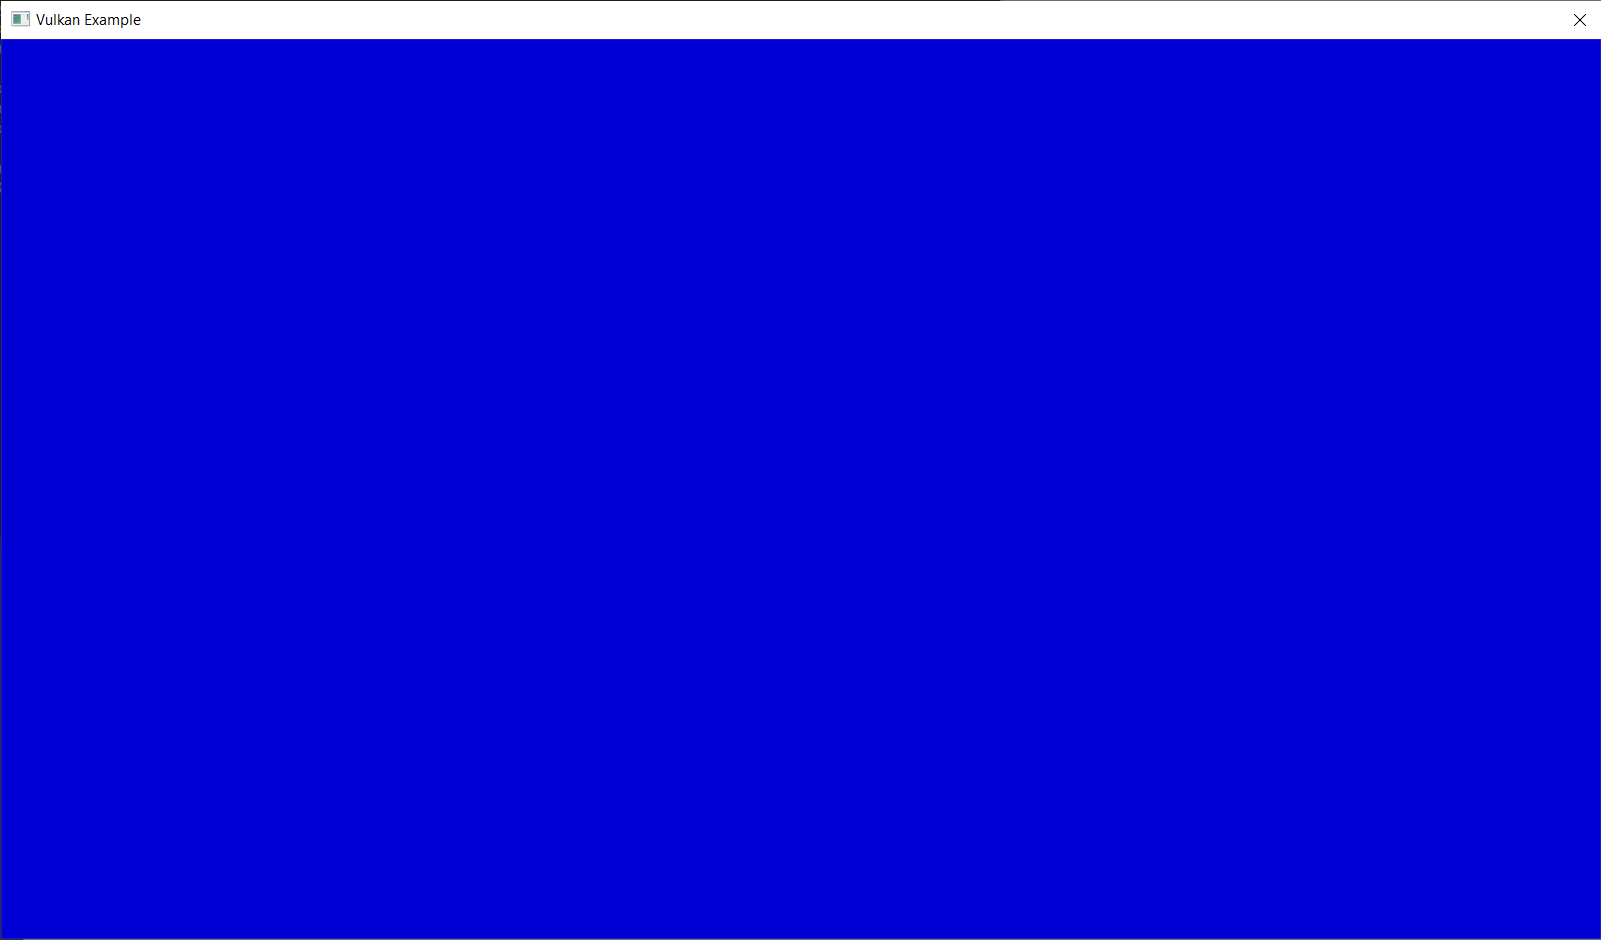
\includegraphics[scale=0.20]{images/ChClearWindow/ClearWindow.png}
    \caption{Clear the window background blue}
    \label{fig::ClearWindow}
\end{figure}

\subsection{Acquire A Swapchain Image}

The first step for drawing something to the screen is to get an image that serves
as our render target.
We also need to be able to present this image to the presentation engine.
Only swapchain images satisfy the latter requirement.
Hence, we must use one of them as our render target.
The problem is that we don't know the next available presentable swapchain image.
To determine such image we use vkAcquireNextImageKHR.
The image is not guaranteed to be already available when the function returns.
For this reason, we use our image available semaphore.
It will be signaled when the image will actually be ready.

\begin{minipage}{\linewidth}{\noindent}
    \lstinputlisting[
        language=C++,
        caption={Acquire the next swapchain image that will be presented},
        label={lst::AcquireNextSwapchainImage}
        ]{src/ChClearWindow/AcquireNextSwapchainImage.cpp}
\end{minipage}

\subsection{Wait For The Previous Commands To Finish}

Before recording new commands into our command buffer, we have to wait for its
execution to finish.
To do this wait for our command buffer fence to be signaled.
After the wait terminates, we have to manually reset our fence state to unsignaled.
We do this so that we can wait on the fence again, during the next frame.

\begin{minipage}{\linewidth}{\noindent}
    \lstinputlisting[
        language=C++,
        caption={Wait for command buffer execution to finish},
        label={lst::CommandBufferWait}
        ]{src/ChClearWindow/CommandBufferWait.cpp}
\end{minipage}

\subsection{Create A Framebuffer}

Before recording our rendering commands, we need to create a new framebuffer.
A framebuffer is the set of attachments that a render pass uses during rendering.
Before creating a new framebuffer, remember to destroy the framebuffer that was used
during the previous frame.
It's also important to remember to destroy the last created framebuffer during
our application cleanup phase.

\begin{minipage}{\linewidth}{\noindent}
    \lstinputlisting[
        language=C++,
        caption={Create a new framebuffer},
        label={lst::CreateFramebuffer}
        ]{src/ChClearWindow/CreateFramebuffer.cpp}
\end{minipage}

\subsubsection{VkFramebufferCreateInfo}

To configure the framebuffer we are about to create we use a VkFramebufferCreateInfo
struct.
In our case, our framebuffer will contain a single attachment: the next
available presentable swapchain image.

\begin{minipage}{\linewidth}{\noindent}
    \lstinputlisting[
        language=C++,
        caption={Configure our framebuffer},
        label={lst::VkFramebufferCreateInfo}
        ]{src/ChClearWindow/VkFramebufferCreateInfo.cpp}
\end{minipage}

\subsection{Record Rendering Commands}

Now we can start recording our new rendering commands.
All the functions that write a command into our command buffer must lay
between vkBeginCommandBuffer and vkEndCommandBuffer.

\begin{minipage}{\linewidth}{\noindent}
    \lstinputlisting[
        language=C++,
        caption={Boilerplate code for recording a command buffer},
        label={lst::BeginEndCommandBuffer}
        ]{src/ChClearWindow/BeginEndCommandBuffer.cpp}
\end{minipage}

Here we are recording a one time submit command buffer.
It means that each recording will only be submitted once to the GPU.
Indeed, for every frame, we record and then submit our command buffer.
Hence, each recording will be submitted only once.
We do this so that we can change our clear color over time.

\begin{minipage}{\linewidth}{\noindent}
    \lstinputlisting[
        language=C++,
        caption={Change window clear color over time},
        label={lst::ComputeClearColor}
        ]{src/ChClearWindow/ComputeClearColor.cpp}
\end{minipage}

Now we can actually write some commands into our command buffer.
The idea is very simple.
We record two commands: the first is for starting an instance of our render pass;
the second is for ending our render pass instance.

\begin{minipage}{\linewidth}{\noindent}
    \lstinputlisting[
        language=C++,
        caption={Clear the window using a render pass},
        label={lst::RenderPassClearScreen}
        ]{src/ChClearWindow/RenderPassClearScreen.cpp}
\end{minipage}

First we have to configure the render pass instance using a VkRenderPassBeginInfo
struct.
The field that requires an explanation is pClearValues.
This is an array of clear values for each attachment.
The array is indexed by attachment number.
Consider the i-th attachment.
If it has \texttt{VK\_ATTACHMENT\_LOAD\_OP\_CLEAR}
as loadOp value, then pClearValues[i] will be used for the clear value.
Otherwise, pClearValues[i] will be ignored.
We use the clear color we computed earlier as our clear value.

\begin{minipage}{\linewidth}{\noindent}
    \lstinputlisting[
        language=C++,
        caption={Configure our render pass instance},
        label={lst::VkRenderPassBeginInfo}
        ]{src/ChClearWindow/VkRenderPassBeginInfo.cpp}
\end{minipage}

Now we can explain how we clear the image with our clear value.
We start by beginning our render pass.
This causes the first subpass to start.
Right before the start of our subpass, an implicit image layout transition occurs.
This causes the swapchain image to transition to
\texttt{VK\_IMAGE\_LAYOUT\_COLOR\_ATTACHMENT\_OPTIMAL}.
With this layout, we can write color data into the image.
Since our subpass is the first to use our swapchain image color attachment, the image
is cleared using the specified clear value.
Right before ending the render pass, another implicit image layout transition occurs.
This causes the swapchain image to transition to
\texttt{VK\_IMAGE\_LAYOUT\_PRESENT\_SRC\_KHR}.
With this layout, our image can be used by the presentation engine.

\subsection{Submit Rendering Commands}

Once we have recorded all the necessary rendering commands into our command
buffer, we can submit it to our GPU for execution.
In our case, we submit the command buffer to the graphics queue.
When the execution of the command buffer is complited, our command buffer fence
will be signaled.

\begin{minipage}{\linewidth}{\noindent}
    \lstinputlisting[
        language=C++,
        caption={Submit command buffer to the GPU},
        label={lst::SubmitCommandBuffer}
        ]{src/ChClearWindow/SubmitCommandBuffer.cpp}
\end{minipage}

We use a VkSubmitInfo struct to configure our command buffer submission.

pWaitSemaphores is an array of semaphores upon which to wait before the submitted
command buffers begin execution.
In our case we only use one semaphore: our image available semaphore.
We do this because we have to wait for our swapchain image to be
available before rendering into it.

pWaitDstStageMask is a bitmask of pipeline stages at which each corresponding
semaphore wait will occur.
In our case we are saying that we do our semaphore wait as soon as the graphics
pipeline starts executing the commands recorded into our command buffer.

pSignalSemaphores is an array of semaphores to be signaled once the submitted command
buffers have completed execution.
In our case we signal only one semaphore: our render finished semaphore.
When this semaphore is signaled, it means that we have finished rendering our
image.

\begin{minipage}{\linewidth}{\noindent}
    \lstinputlisting[
        language=C++,
        caption={Configure command buffer submission},
        label={lst::VkSubmitInfo}
        ]{src/ChClearWindow/VkSubmitInfo.cpp}
\end{minipage}

\subsection{Present}

The only thing missing is to actually present our rendered image to the window.
Here we specify our present queue as the GPU queue that will execute our present
command.

\begin{minipage}{\linewidth}{\noindent}
    \lstinputlisting[
        language=C++,
        caption={Issue a present command},
        label={lst::Present}
        ]{src/ChClearWindow/Present.cpp}
\end{minipage}

We use a VkPresentInfoKHR struct to configure our present command submission.

pWaitSemaphores is an array of semaphores to wait for before issuing the present
command.
In our case we only use one semaphore: our render finished semaphore.
Simply put, we have to wait for our rendering to finish before presenting
the image to the window.

\begin{minipage}{\linewidth}{\noindent}
    \lstinputlisting[
        language=C++,
        caption={Configure present command submission},
        label={lst::VkPresentInfoKHR}
        ]{src/ChClearWindow/VkPresentInfoKHR.cpp}
\end{minipage}

\section{Cleanup}

Now that our application submits commands to the GPU, a problem may arise.
Being commands executed asynchronously on the GPU, we could exit the application,
and thus freeing all our resources, before all submitted commands finish
their execution.
This can lead to errors, because some commands may act upon one or more resources
that were deleted.
We can fix this issue by waiting for our device to be idle, meaning that
all processing on all device's queues is finished, before cleaning up our resources.
We can do this using vkDeviceWaitIdle.

\section{Our Application So Far}

Here we can see how all the concepts we have seen in this chapter come together
to form our application

\begin{minipage}{\linewidth}{\noindent}
    \lstinputlisting[
        language=C++,
        caption={Structure of our application},
        label={lst::ChClearWindowApp}
        ]{src/ChClearWindow/Application.cpp}
\end{minipage}
